\documentclass[11pt,a4paper]{article}
\usepackage[margin=1.8cm]{geometry}
\usepackage{xcolor}
\usepackage{amssymb}
\usepackage{graphicx}
\usepackage[most]{tcolorbox}
\usepackage{array,tabularx,booktabs}
\usepackage{enumitem}
\usepackage{fontspec}
\usepackage{polyglossia}
\setdefaultlanguage{french}
\setotherlanguage{arabic}
\setmainfont{DejaVu Serif}
\newfontfamily\arabicfont[Script=Arabic,Scale=1.05]{DejaVu Sans}
\newfontfamily\arabicfontsf[Script=Arabic,Scale=1.05]{DejaVu Sans}
\graphicspath{{img/}}
\setlength{\parindent}{0pt}
\setlength{\parskip}{4pt}
\renewcommand{\arraystretch}{1.35}
\setlist{itemsep=2pt,topsep=3pt}

\definecolor{bleu}{HTML}{2E5C9A}
\definecolor{vert}{HTML}{2E7D32}
\definecolor{rouge}{HTML}{C62828}
\definecolor{orange}{HTML}{E65100}
\definecolor{gris}{HTML}{455A64}
\definecolor{violet}{HTML}{6A1B9A}
\definecolor{teal}{HTML}{00695C}

\newtcolorbox{carte}{colback=bleu!6,colframe=bleu,title=Où on est sur la carte,fonttitle=\bfseries}
\newtcolorbox{examen}{colback=vert!6,colframe=vert,title=Phrases d'examen à connaître (en français),fonttitle=\bfseries}
\newtcolorbox{piege}{colback=rouge!5,colframe=rouge,title=Pièges des examens,fonttitle=\bfseries}
\newtcolorbox{resume}{colback=orange!6,colframe=orange,title=Résumé en 3 phrases,fonttitle=\bfseries}
\newtcolorbox{note}{colback=gris!6,colframe=gris,title=Note / Astuce,fonttitle=\bfseries}
\newtcolorbox{alerte}{colback=violet!5,colframe=violet,title=Alerte : les sources ne sont pas d'accord,fonttitle=\bfseries}
\newtcolorbox{exemple}{colback=teal!5,colframe=teal,title=Exemple,fonttitle=\bfseries}

\newcommand{\ar}[1]{\textarabic{#1}}
\newcommand{\fr}[1]{\textfrench{#1}}
\newcommand{\vrai}{\textcolor{vert}{\textbf{VRAI}}}
\newcommand{\faux}{\textcolor{rouge}{\textbf{FAUX}}}
\newcommand{\partie}[1]{\newpage\section*{#1}\addcontentsline{toc}{section}{#1}}

\begin{document}

%======================================================================
\begin{center}
{\LARGE\bfseries Systèmes de Production}\\[4pt]
{\Large Chapitre 1 : du produit à l'usine}\\[4pt]
{\large Fiche de révision (arabe + français)}\\[2pt]
{\small Basée sur le cours (BARABAS), le TD1 et les tests 2022-23, 2023-24, 2024-25}
\end{center}

\section*{0. La carte du chapitre}

\par\begin{Arabic}
\textbf{الفكرة ديال الكورس كاملة فجملة وحدة:}
شركة بغات تصنع منتوج جديد. شنو خاصها تدير من الفكرة حتى للمعمل اللي كيخدم؟
والهدف ديالها ديما هو \textbf{\fr{QCD}}: جودة مزيانة (\fr{Qualité})، بثمن معقول (\fr{Coût})، فالوقت (\fr{Délai}).

\textbf{المثال اللي غادي نتبعو فكل الفيش:} بغيتي تحل \textbf{معمل ديال الدراجات} (\fr{vélos}).
\end{Arabic}

\begin{center}
\begin{tabularx}{\linewidth}{c >{\raggedleft\arraybackslash}X l}
\toprule
\textbf{Partie} & \ar{\textbf{السؤال}} & \textbf{Titre} \\
\midrule
1 & \ar{شنو هو الهدف ديالي؟} & L'idée générale (QCD) \\
2 & \ar{شنو هي الكلمات الأساسية؟} & Concepts de base \\
3 & \ar{كيفاش نصمم الدراجة؟} & Conception de produits (NPD) \\
4 & \ar{أشمن نوع ديال المعمل يناسبني؟} & Classification (4a, 4b, 4c) \\
5 & \ar{كيفاش نختار؟ وكيفاش نحسب؟} & Sélection du processus + calculs \\
6 & \ar{كيفاش نبني المعمل خطوة بخطوة؟} & Conception d'un système de production \\
7 & \ar{كيفاش ندوز من دراجة وحدة لآلاف الدراجات؟} & Industrialisation \\
\bottomrule
\end{tabularx}
\end{center}

\begin{tcolorbox}[colback=bleu!4,colframe=bleu,title=La chaîne logique du chapitre,fonttitle=\bfseries]
\centering
\textbf{Parties 1 + 2} (la base) $\;\longrightarrow\;$ \textbf{Partie 3} (le produit) $\;\longrightarrow\;$ \textbf{Parties 4 + 5} (choisir l'usine)\\[3pt]
$\longrightarrow\;$ \textbf{Partie 6} (construire l'usine) $\;\longrightarrow\;$ \textbf{Partie 7} (produire en série)
\par\begin{Arabic}
\centering
منتوج ← نوع المعمل ← بناء المعمل ← الإنتاج
\end{Arabic}
\end{tcolorbox}

\subsection*{Poids du chapitre 1 dans les examens}
\begin{center}
\begin{tabular}{lccc}
\toprule
\textbf{Source} & \textbf{Total} & \textbf{Chapitre 1} & \textbf{Chapitre 2} \\
\midrule
TD1 & 37 & 24 & 13 \\
Test 2022-23 & 20 & 17 & 3 \\
Test 2023-24 & 38 & 22 & 16 \\
Test 2024-25 & 22 & 15 & 7 \\
\midrule
\textbf{Total} & \textbf{117} & \textbf{78} & \textbf{39} \\
\bottomrule
\end{tabular}
\end{center}
\par\begin{Arabic}
\textbf{يعني:} جوج تلت ديال الأسئلة كيجيو من الفصل 1. والجزء 4 هو اللي كيطيح أكثر.
\end{Arabic}

\subsection*{Comment lire cette fiche}
\begin{itemize}
\item \textcolor{bleu}{\textbf{Bleu}} : où on est et à quoi sert la partie.
\item \textcolor{vert}{\textbf{Vert}} : phrases exactes des examens (à reconnaître en français).
\item \textcolor{rouge}{\textbf{Rouge}} : pièges (VRAI / FAUX).
\item \textcolor{gris}{\textbf{Gris}} : notes et astuces pour retenir.
\item \textcolor{teal}{\textbf{Vert-bleu}} : exemples.
\item \textcolor{violet}{\textbf{Violet}} : alertes quand le TD, le cours et les tests ne disent pas la même chose.
\item \textcolor{orange}{\textbf{Orange}} : résumé à relire la veille de l'examen.
\end{itemize}

\subsection*{Règles du test}
\begin{itemize}
\item QCM de 45 min, \textbf{une ou plusieurs} réponses justes.
\item Réponse fausse : $-0{,}25$ ou $-0{,}5$ point. \ar{ما تكوشيش بالزهر.}
\item Calculs : \textbf{sans chiffre après la virgule} : 62,85 $\rightarrow$ \textbf{62} (on \textbf{tronque}, on n'arrondit pas).
\end{itemize}

%======================================================================
\partie{Parties 1 + 2 : L'idée générale et les concepts de base}

\begin{carte}
\textbf{Parties 1 + 2} $\rightarrow$ 3 $\rightarrow$ 4 $\rightarrow$ 5 $\rightarrow$ 6 $\rightarrow$ 7
\par\begin{Arabic}
\textbf{الدور ديال هاد الجزء:} نعرفو الهدف (\fr{QCD}) والكلمات الأساسية اللي غادي نستعملو فكاع الفصل.
\end{Arabic}
\end{carte}

\subsection*{1. L'idée générale}
Une entreprise doit livrer un produit avec la bonne \textbf{Qualité}, au bon \textbf{Coût}, dans les bons \textbf{Délais} : c'est le triangle \textbf{QCD}. Pour cela :
\begin{enumerate}
\item \textbf{concevoir le produit} (NPD) ;
\item \textbf{choisir et concevoir le système de production} ;
\item \textbf{industrialiser} : passer du prototype à la série.
\end{enumerate}

\subsection*{2. Les 3 définitions à ne pas confondre \quad (tombe à chaque test)}
\begin{center}
\begin{tabularx}{\linewidth}{l X l}
\toprule
\textbf{Terme} & \textbf{Définition} & \textbf{Exemple} \\
\midrule
Produit & Bien ou service qui satisfait un client & le vélo \\
Processus & Ensemble de ressources reliées par un flux de matière, transformant les intrants en extrants & la ligne de peinture \\
Système de production & Ensemble organisé de moyens \textbf{humains, matériels, technologiques, financiers, informationnels} pour atteindre le \textbf{QCD} & toute l'usine \\
\bottomrule
\end{tabularx}
\end{center}

\begin{examen}
\begin{itemize}
\item « Un système de production est un processus d'ajout de valeur à des biens ou à des services. » \vrai
\item « Un ensemble de moyens humains et matériels qui collaborent pour atteindre les objectifs QCD de la fonction industrielle. » \vrai
\item « Tout ce qui prend des entrées et les transforme en sorties avec une valeur ajoutée. » \vrai
\item « Un ensemble de processus qui transforment des ressources en produits ou services finis. » \vrai
\item « Un processus est un ensemble de ressources reliées par un flux de matière, transformant les intrants en extrants. » \vrai
\end{itemize}
\end{examen}

\begin{piege}
\begin{itemize}
\item « Est composé \textbf{uniquement} de processus principaux. » \faux
\item « Permet de répondre \textbf{uniquement} aux objectifs de la fonction maintenance. » \faux
\item « Système qui prévoit le besoin d'un client. » \faux
\item « Tout ce qui commercialise le produit dans l'entreprise. » \faux
\item « Une combinaison de moyens techniques et humains permettant de \textbf{gérer les opérations}. » \faux \ (test 2024-25)
\item « Un processus est un ensemble de machines. » \faux
\end{itemize}
\end{piege}

\begin{note}
\par\begin{Arabic}
\textbf{القاعدة:} الكلمة \textbf{« \fr{uniquement} »} ديما كتعني أن الجواب \textbf{غالط}.
ونظام الإنتاج كي\textbf{حول} (\fr{transforme}) وكيزيد القيمة، ماشي غير كي\textbf{سير} (\fr{gérer}).
\end{Arabic}
\end{note}

\subsection*{3. Efficace vs efficient}
\par\begin{Arabic}
\begin{itemize}
\item \textbf{\fr{Efficace}}: كتوصل للهدف، ولو صرفتي بزاف.
\item \textbf{\fr{Efficient}}: كتوصل للهدف \textbf{بأقل} حاجة (وقت، مادة، طاقة، فلوس). صفر تبذير.
\end{itemize}
\end{Arabic}
\begin{exemple}
Deux boulangers font chacun 100 pains de bonne qualité (\textbf{efficaces} tous les deux). Le premier jette 20 kg de farine, le second rien : seul le second est \textbf{efficient}. Un système de production doit être \textbf{les deux}.
\end{exemple}

\subsection*{4. Les 3 types de processus}
\begin{center}
\begin{tabularx}{\linewidth}{l X >{\raggedleft\arraybackslash}X}
\toprule
\textbf{Processus} & \textbf{Rôle} & \ar{\textbf{بالدارجة}} \\
\midrule
Pilotage & Décide et dirige : stratégie, qualité & \ar{كيقرر وكيسير} \\
Réalisation & Transforme réellement le produit & \ar{كيصنع المنتوج بصح} \\
Support & Aide : maintenance, méthodes, RH, bureau d'études, budget & \ar{كيعاون الآخرين} \\
\bottomrule
\end{tabularx}
\end{center}
\par\begin{Arabic}
\textbf{علاش « \fr{uniquement de processus principaux} » غالطة؟} حيت كاين حتى \fr{pilotage} و\fr{support}.
\end{Arabic}

\subsection*{5. Les 3 flux de l'entreprise}
\begin{center}
\begin{tabularx}{\linewidth}{l X}
\toprule
\textbf{Flux} & \textbf{Contenu} \\
\midrule
Physique (matière) & matière première $\rightarrow$ en-cours $\rightarrow$ produit fini \\
Information & \textbf{commande client} $\rightarrow$ ordre de fabrication (OF) $\rightarrow$ commande matière \\
Financier (argent) & clients $\rightarrow$ banques $\rightarrow$ fournisseurs et personnel \\
\bottomrule
\end{tabularx}
\end{center}

\begin{note}
\par\begin{Arabic}
\textbf{الفلوكس ديال المعلومات كيبدا ديما من الزبون:} الزبون كيطلب ← كنعطيو أمر التصنيع (\fr{OF}) ← كنشريو المادة.
\end{Arabic}
\end{note}

\begin{piege}
\begin{itemize}
\item « Flux matière, flux d'argent et flux informationnel. » \vrai
\item « Flux tiré, flux poussé et flux tendu. » \faux \ \ar{(هادو ماشي أنواع ديال الفلوكس، هادو طرق ديال التسيير)}
\item « Flux par quantité et flux par variété. » \faux
\end{itemize}
\end{piege}

\par\begin{Arabic}
\textbf{تيري، پوسي، تاندو:} هادو \textbf{طرق ديال تسيير الإنتاج}:
\end{Arabic}
\begin{center}
\begin{tabular}{lll}
\toprule
\textbf{Mode} & \textbf{Signification} & \textbf{Lien} \\
\midrule
Flux \textbf{tiré} (pull) & on produit sur \textbf{commande client} & MTO \\
Flux \textbf{poussé} (push) & on produit sur \textbf{prévision} & MTS \\
Flux \textbf{tendu} & juste à temps, zéro stock & JIT \\
\bottomrule
\end{tabular}
\end{center}
\begin{examen}
« En général, le stock est placé dans le point d'intersection du flux tiré et du flux poussé. » \vrai \ (TD Q9d)
\par\begin{Arabic}
يعني: الستوك كيتحط فالبلاصة اللي كيتلاقاو فيها التوقعات (\fr{poussé}) مع الطلبية ديال الزبون (\fr{tiré}). هادي كتسمى \fr{point de découplage}.
\end{Arabic}
\end{examen}

\subsection*{6. La boucle de régulation}
On \textbf{mesure} la sortie, on la \textbf{compare} à l'objectif, on \textbf{corrige} : c'est la rétroaction (\emph{feedback}). Peu testé.

\subsection*{7. Sigles utiles}
\begin{center}
\begin{tabularx}{\linewidth}{l X}
\toprule
ISO 9001 & \textbf{qualité} \\
ISO 14001 & \textbf{environnement} \\
ISO 45001 & \textbf{santé et sécurité au travail} \ \ar{(غلطتي فيها فالـ QCM، ركز!)} \\
3R & Réduire, Réutiliser, Recycler \\
3 piliers du développement durable & environnemental, social, économique \\
SdF & sûreté de fonctionnement : fiabilité, disponibilité, maintenabilité \\
OF / OA / PIC & ordre de fabrication / ordre d'achat / plan industriel et commercial \\
PLM & Product Lifecycle Management \\
OMPIC & Office marocain de la propriété industrielle (brevets) \\
Transport vs manutention & transport = entre ateliers ou vers l'extérieur ; manutention = du stock au poste de travail \\
\bottomrule
\end{tabularx}
\end{center}

\begin{resume}
\begin{enumerate}
\item Système de production = moyens humains et matériels qui \textbf{transforment} pour atteindre le \textbf{QCD}.
\item 3 processus : pilotage, réalisation, support. 3 flux : matière, information, argent.
\item Tiré = MTO, poussé = MTS, tendu = JIT. Le mot « uniquement » = piège.
\end{enumerate}
\end{resume}

\subsection*{Mini-QCM}
\begin{enumerate}
\item La maintenance et les RH sont des processus : (a) de pilotage (b) de réalisation (c) de support
\item Atteindre l'objectif avec le minimum de ressources : (a) efficace (b) efficient
\item Norme santé et sécurité au travail : (a) ISO 9001 (b) ISO 14001 (c) ISO 45001
\item Ordre du flux d'information : (a) matière $\rightarrow$ OF $\rightarrow$ client (b) client $\rightarrow$ OF $\rightarrow$ matière
\item Flux poussé correspond à : (a) MTO (b) MTS (c) JIT
\end{enumerate}
{\small\textit{Réponses : 1-c, 2-b, 3-c, 4-b, 5-b.}}

%======================================================================
\partie{Partie 3 : Conception de produits (NPD)}

\begin{carte}
1 + 2 \checkmark\ $\rightarrow$ \textbf{Partie 3} $\rightarrow$ 4 $\rightarrow$ 5 $\rightarrow$ 6 $\rightarrow$ 7
\par\begin{Arabic}
\textbf{الدور ديال هاد الجزء:} قبل ما نبنيو المعمل، خاصنا نعرفو \textbf{شنو غادي نصنعو}. هنا كنصممو الدراجة من الفكرة حتى للنموذج التجريبي.
\end{Arabic}
\end{carte}

\subsection*{1. Pourquoi c'est crucial}
\par\begin{Arabic}
السوق كيتبدل بزربة والمنافسة كبيرة. إذن:
\begin{itemize}
\item خاصك تخرج المنتوج \textbf{بزربة}: الـ \fr{Time To Market} خاصو يكون \textbf{قصير}.
\item المنتوجات كتعيش \textbf{وقت قصير} فالسوق.
\item خاصك \textbf{تبتكر وتتميز} على المنافسين.
\end{itemize}
\end{Arabic}
\begin{piege}
\begin{itemize}
\item « Les sociétés ont intérêt à avoir un time to market de plus en plus \textbf{grand}. » \faux
\item « Le cycle de vie des produits devient de plus en plus \textbf{court}. » \vrai
\end{itemize}
\end{piege}

\subsection*{2. Cycle de vie d'un produit}
\begin{center}
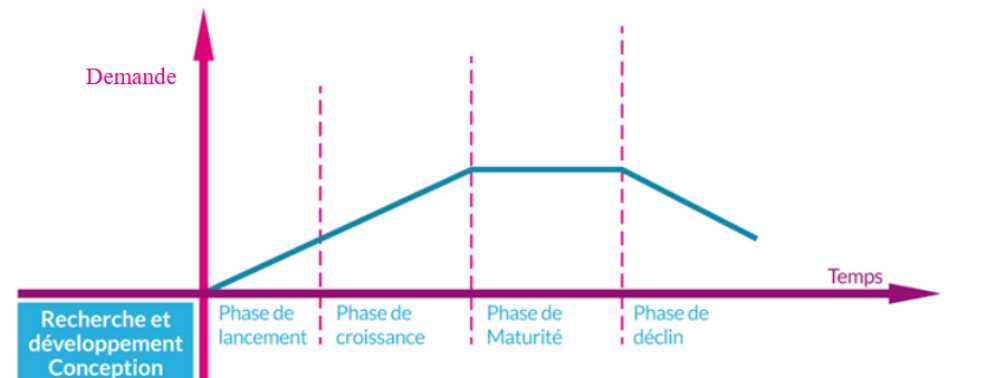
\includegraphics[width=0.7\linewidth]{cycle_vie}
\end{center}
\par\begin{Arabic}
بحال حياة الإنسان: كيتصمم ← كيخرج للسوق ← كيكبر ← كيستقر ← كينقص.
\end{Arabic}
\begin{examen}
\textbf{Développement $\rightarrow$ Lancement $\rightarrow$ Croissance $\rightarrow$ Maturité $\rightarrow$ Déclin} \vrai\\
« Introduction, développement, croissance, maturité et déclin » \faux \ (test 2023-24)
\end{examen}

\subsection*{3. Conception à coût objectif (CCO, design to cost)}
\par\begin{Arabic}
\textbf{70\% من الثمن كيتقرر فالتصميم.}
\begin{itemize}
\item غلطة فالتصنيع ← كتأثر غير على قطعة ولا مجموعة صغيرة.
\item غلطة فالتصميم ← كتأثر على \textbf{كاع} المنتوجات. إلا ما شفتيهاش بكري، كتكلف بزاف (تبديل الأدوات، إعادة القطع…).
\end{itemize}
إذن: \textbf{فكر فالتكلفة من النهار الأول}.
\end{Arabic}
On réduit les coûts en agissant sur : matière première, forme du produit, nombre de pièces, simplification des processus, énergie.
\begin{examen}
\begin{itemize}
\item « Une approche de conception qui vise à réduire les coûts de production dès le début du processus de conception. » \vrai
\item « La méthode design to cost consiste à intégrer les contraintes de coût dès la phase de conception du produit. » \vrai
\end{itemize}
\end{examen}
\begin{piege}
« Réduit le nombre de fonctionnalités » \faux \quad « Ne se préoccupe pas des coûts » \faux
\end{piege}

\subsection*{4. Les 6 étapes du NPD (Ulrich \& Eppinger) \quad (tombe dans les 4 sources)}
\begin{center}
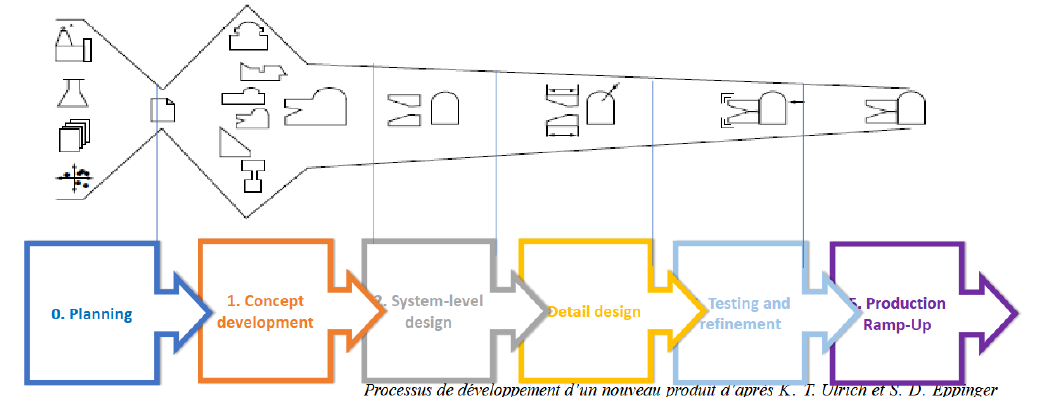
\includegraphics[width=0.8\linewidth]{npd_6_etapes}
\end{center}
\begin{center}
\begin{tabularx}{\linewidth}{l >{\raggedleft\arraybackslash}X l}
\toprule
\textbf{Étape} & \ar{\textbf{بالدارجة}} & \textbf{Résultat} \\
\midrule
0. Planification & \ar{واش المشروع ممكن؟} & énoncé de mission (kick-off) \\
1. Développement du \textbf{concept} & \ar{كنرسم \textbf{بزاف ديال الأفكار} وكنختار المزيانة} & un concept \\
2. Conception \textbf{préliminaire} & \ar{كنقسم الدراجة لأجزاء: \fr{architecture}} & plan initial + maquette \\
3. Conception \textbf{détaillée} & \ar{كل قطعة: الشكل، المادة، القياسات} & documentation complète \\
4. Test et raffinement & \ar{كنجرب وكنصلح} & produit fiable \\
5. Montée en cadence & \ar{كنبدا الإنتاج بالكمية الكبيرة} & production en masse \\
\bottomrule
\end{tabularx}
\end{center}

\begin{examen}
\begin{itemize}
\item « Lors du développement des concepts, plusieurs produits (concepts) alternatifs sont générés. » \vrai
\item « La conception préliminaire consiste en la définition de l'architecture du produit. » \vrai
\item « La conception préliminaire se fait \textbf{après} le développement du concept. » \vrai
\item « La conception détaillée : définition des spécifications techniques précises et des dessins techniques. » \vrai
\end{itemize}
\end{examen}
\begin{piege}
\begin{itemize}
\item « La conception préliminaire consiste à générer plusieurs concepts. » \faux \ \ar{(هادا \fr{concept})}
\item « La conception préliminaire consiste en la définition de la forme, des matériaux et des tolérances. » \faux \ \ar{(هادا \fr{détaillée})}
\item « La conception préliminaire se fait \textbf{avant} le développement du concept. » \faux
\item « L'étape de développement des concepts consiste en la définition de l'architecture. » \faux
\end{itemize}
\end{piege}
\begin{note}
\par\begin{Arabic}
\textbf{باش تتفكر:} بزاف ديال الأفكار = \fr{concept} \quad|\quad الأجزاء الكبار = \fr{préliminaire} \quad|\quad كل قطعة بالتفصيل = \fr{détaillée}
\end{Arabic}
\end{note}

\subsection*{5. Maquette, prototype alpha, présérie \quad (tombe dans les 4 sources)}
\begin{center}
\begin{tabularx}{\linewidth}{l X l}
\toprule
\textbf{Type} & \textbf{Description} & \textbf{Procédé} \\
\midrule
Maquette & non fonctionnelle, montre la forme et l'esthétique ; la \textbf{maquette numérique} teste les concepts avant le physique & -- \\
Prototype \textbf{alpha} & \textbf{même forme et même matériau} que le produit final ; valide la faisabilité, la géométrie et le matériau & \textbf{différent} \\
\textbf{Présérie} (bêta) & petite quantité, pour tester le \textbf{processus} et la \textbf{qualité} avant la série & \textbf{final} \\
\bottomrule
\end{tabularx}
\end{center}
\par\begin{Arabic}
\textbf{بالدارجة:} \fr{alpha} = دراجة بنفس الشكل والمادة، ولكن مصنوعة \textbf{بطريقة أخرى} (باليد مثلا). \fr{Présérie} = دراجات مصنوعين \textbf{بنفس الطريقة ديال المعمل}، ولكن شوية باش نجربو.
\end{Arabic}
\begin{piege}
\begin{itemize}
\item « Les prototypes de présérie ne sont \textbf{jamais} réalisés par le processus prévu. » \faux
\item « Les prototypes de présérie doivent être réalisés par le processus de production prévu. » \vrai
\item « Les premiers prototypes ne doivent \textbf{pas} avoir la même forme et les mêmes matériaux. » \faux
\item « Un prototype alpha est fabriqué dans les mêmes conditions que la production de masse. » \faux
\item « Les tests sur prototypes Beta se font \textbf{uniquement après} la mise sur le marché. » \faux
\item « Les maquettes numériques permettent de tester des concepts avant le prototypage physique. » \vrai
\item « Rôle de l'alpha : valider la géométrie et les propriétés de matériau. » \vrai
\end{itemize}
\end{piege}
Ressources mobilisées (peu testé) : documentaires (normes), humaines (ingénieurs), informatiques (CAO, PLM), techniques (bancs d'essai, prototypage rapide).

\subsection*{6. Innovation et brevet}
\par\begin{Arabic}
\begin{itemize}
\item \textbf{\fr{Innovation}} = اختراع \textbf{نجح فالسوق}. (العكس غالط!)
\item \textbf{\fr{Brevet}}: الدولة كتعطيك \textbf{الحق وحدك} تستغل الاختراع ديالك، \textbf{لمدة محدودة}.
\item الشروط: جديد، فيه ابتكار، وقابل للتطبيق فالصناعة.
\item فالمغرب: \textbf{\fr{OMPIC}}.
\item بعض الشركات \textbf{كتخبي السر} بلا براءة (\fr{Coca-Cola}، \fr{Google}، \fr{Michelin})، حيت البراءة كتفرض تنشر الاختراع.
\end{itemize}
\end{Arabic}
\textbf{Dépôt en 4 étapes :} (1) dépôt du dossier ; (2) examen par la \textbf{défense nationale} (secret ?) ; (3) examen par la propriété industrielle (antériorité) ; (4) délivrance.

\textbf{5 niveaux d'inventivité :} solution apparente $\rightarrow$ amélioration mineure $\rightarrow$ amélioration majeure $\rightarrow$ nouveau concept $\rightarrow$ découverte scientifique.

\begin{piege}
\begin{itemize}
\item « Une invention est une innovation adoptée par le marché. » \faux \ \ar{(قلبوها)}
\item « Le brevet sert à protéger la propriété industrielle d'une invention. » \vrai
\item « Le brevet sert à protéger la marque d'un produit. » \faux
\item « Le brevet sert à protéger les secrets de fabrication. » \faux
\item « Les entreprises choisissent parfois de garder leurs innovations secrètes. » \vrai
\item « La demande de brevet est examinée par la défense nationale. » \vrai
\item « La validité d'un brevet est limitée dans le temps. » \vrai
\end{itemize}
\end{piege}

\begin{resume}
\begin{enumerate}
\item Penser au coût dès la conception (70\%) ; time to market \textbf{court}.
\item Concept (plusieurs idées) $\rightarrow$ préliminaire (architecture) $\rightarrow$ détaillée (forme, matériaux, tolérances).
\item Alpha = autre procédé ; présérie = procédé final.
\end{enumerate}
\end{resume}

\subsection*{Mini-QCM}
\begin{enumerate}
\item La conception préliminaire consiste en : (a) générer plusieurs concepts (b) l'architecture (c) forme, matériaux, tolérances
\item Le prototype alpha : (a) procédé final (b) même forme et matériau, autre procédé (c) non fonctionnel
\item Cycle de vie : (a) introduction, développement\ldots\ (b) développement, lancement, croissance, maturité, déclin
\item Pour être compétitive, une entreprise doit : (a) augmenter (b) réduire son time to market
\item La présérie est fabriquée : (a) avec le procédé final (b) jamais avec le procédé final
\end{enumerate}
{\small\textit{Réponses : 1-b, 2-b, 3-b, 4-b, 5-a.}}

%======================================================================
\partie{Partie 4a : Combien on produit ? (Quantité / Variété)}

\begin{carte}
3 \checkmark\ $\rightarrow$ \textbf{4a} $\rightarrow$ 4b (implantations) $\rightarrow$ 4c (MTS / MTO) $\rightarrow$ 5 $\rightarrow$ 6 $\rightarrow$ 7
\par\begin{Arabic}
\textbf{الدور ديال هاد الجزء:} الدراجة مصممة. دابا خاصنا نعرفو أشمن نوع ديال المعمل غادي نحتاجو.
وأول سؤال هو: \textbf{شحال من دراجة غادي نصنعو؟ ونوع واحد ولا بزاف ديال الأنواع؟}
\end{Arabic}
\end{carte}

\begin{note}
\par\begin{Arabic}
الجزء 4 فيه \textbf{8 معايير} باش نصنفو المعامل. قسمناهم على 3: \textbf{4a} شحال كنصنعو، \textbf{4b} كيفاش كنرتبو الماكينات، \textbf{4c} إمتى كنصنعو.
\end{Arabic}
\end{note}

\subsection*{1. La quantité (volume)}
\begin{center}
\begin{tabular}{lll}
\toprule
\textbf{Type} & \textbf{Quantité} & \textbf{Exemple} \\
\midrule
Unitaire & 1 pièce & bateau \\
Par lots (batch) & lots successifs & \\
Petite série & $< 100$ & vélos de course spéciaux \\
Moyenne série & $100$ à $10\,000$ & \\
Grande série & $> 10\,000$ & vélos normaux \\
Production de masse & très grands volumes & bouteilles d'eau \\
\bottomrule
\end{tabular}
\end{center}

\subsection*{2. La variété}
\par\begin{Arabic}
التنوع هو \textbf{شحال من نوع} ديال المنتوج كتصنع (لون، حجم، موديل…).

\textbf{القاعدة الذهبية:}
\begin{itemize}
\item \textbf{كمية كبيرة} ← \textbf{تنوع قليل} (بزاف ديال الدراجات بنفس الموديل)
\item \textbf{كمية صغيرة} ← \textbf{تنوع كبير} (شوية ديال الدراجات، وكل وحدة مختلفة)
\end{itemize}
\end{Arabic}
\begin{examen}
« La variété est en \textbf{corrélation inverse} avec la quantité. »\\
« Moins la variété des produits est grande, plus la quantité est grande. » \vrai
\end{examen}

\subsection*{3. La répétitivité}
\begin{itemize}
\item \textbf{Répétitif} : produits standardisés, en grande quantité.
\item \textbf{Non répétitif} : produits uniques ou petites séries, souvent personnalisés, grande variété.
\end{itemize}

\subsection*{4. Productivité et flexibilité \quad (tombe à chaque test)}
\par\begin{Arabic}
جوج كلمات خاصك تفهمهم مزيان:
\begin{itemize}
\item \textbf{\fr{Productivité}} (الإنتاجية) = تصنع \textbf{بزاف} بزربة ← مرتبطة بـ\textbf{الكمية}
\item \textbf{\fr{Flexibilité}} (المرونة) = تقدر \textbf{تتأقلم} بسهولة (منتوج جديد، كمية مختلفة) ← مرتبطة بـ\textbf{التنوع}
\end{itemize}
ما يمكنش يكون عندك جوج بزاف فنفس الوقت.
\end{Arabic}
\begin{examen}
\begin{itemize}
\item « Plus on gagne en productivité, plus on perd en flexibilité. »
\item « La flexibilité est la capacité à s'adapter rapidement aux changements, comme la variation du volume de production ou le changement de produit. » \vrai
\item « La flexibilité est essentielle en petite série pour s'adapter aux changements de produits. » \vrai
\item « Pour produire une grande variété, il faut opter pour un système flexible FMS. » \vrai
\end{itemize}
\end{examen}

\begin{center}
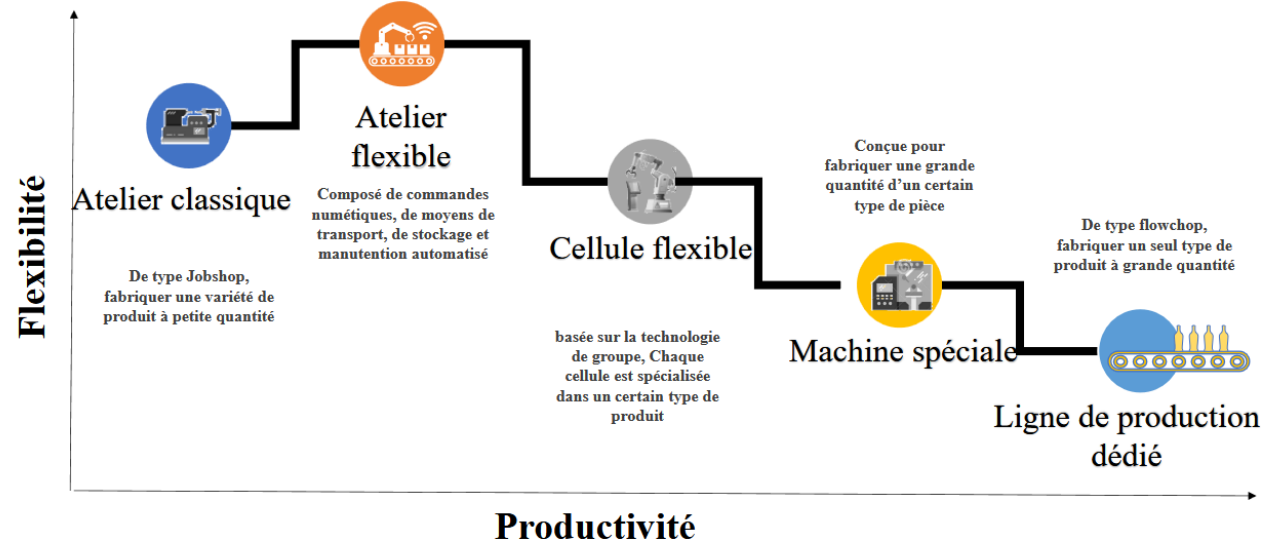
\includegraphics[width=0.85\linewidth]{productivite_flexibilite}
\end{center}
\begin{center}
\begin{tabularx}{\linewidth}{l >{\raggedleft\arraybackslash}X c c}
\toprule
\textbf{Système} & \textbf{Description} & \textbf{Flexibilité} & \textbf{Productivité} \\
\midrule
Atelier classique & \ar{ماكينات عادية، كل مرة حاجة مختلفة (\fr{job shop})} & élevée & faible \\
Atelier flexible (FMS) & \ar{ماكينات رقمية + نقل وتخزين أوتوماتيكي + تسيير بالحاسوب} & très élevée & moyenne \\
Cellule flexible & \ar{مجموعة ماكينات لعائلة وحدة ديال القطع (\fr{technologie de groupe})} & moyenne & moyenne / élevée \\
Machine spéciale & \ar{ماكينة لنوع واحد ديال القطع بكمية كبيرة} & faible & élevée \\
Ligne dédiée & \ar{خط إنتاج لمنتوج واحد بكمية ضخمة (\fr{flow shop})} & très faible & très élevée \\
\bottomrule
\end{tabularx}
\end{center}

\begin{piege}
\begin{itemize}
\item « Plus la variété est grande, plus la quantité est grande. » \faux
\item « La variété et la quantité sont indépendantes. » \faux
\item « Le nombre de différents types de produits quantifie la productivité. » \faux \ \ar{(التنوع = \fr{flexibilité})}
\item « La quantité de produits quantifie la flexibilité. » \faux \ \ar{(الكمية = \fr{productivité})}
\item « On choisit le type de système de production selon les deux critères productivité et flexibilité. » \vrai
\item « Produire en grandes quantités permet systématiquement d'offrir une large variété. » \faux
\item « Une cellule flexible est plus flexible qu'un atelier flexible. » \faux
\end{itemize}
\end{piege}

\begin{resume}
\begin{enumerate}
\item Quantité grande $\Rightarrow$ variété faible (corrélation inverse).
\item Quantité $\rightarrow$ productivité \quad / \quad Variété $\rightarrow$ flexibilité.
\item Plus on gagne en productivité, plus on perd en flexibilité.
\end{enumerate}
\end{resume}

\subsection*{Mini-QCM}
\begin{enumerate}
\item Relation variété / quantité : (a) plus de variété = plus de quantité (b) moins de variété = plus de quantité (c) indépendantes
\item Le nombre de types de produits quantifie : (a) la productivité (b) la flexibilité (c) la qualité
\item Le système le plus productif : (a) atelier classique (b) cellule flexible (c) ligne dédiée
\item Une moyenne série : (a) $<100$ (b) $100$ à $10\,000$ (c) $>10\,000$
\end{enumerate}
{\small\textit{Réponses : 1-b, 2-b, 3-c, 4-b.}}

%======================================================================
\partie{Partie 4b : Comment on range les machines ? (Implantations)}

\begin{carte}
4a \checkmark\ $\rightarrow$ \textbf{4b} $\rightarrow$ 4c $\rightarrow$ 5 $\rightarrow$ 6 $\rightarrow$ 7
\par\begin{Arabic}
\textbf{الدور ديال هاد الجزء:} عرفنا شحال غادي نصنعو. دابا كنقررو \textbf{كيفاش نحطو الماكينات فالمعمل}. هاد الترتيب كيتسمى \textbf{\fr{implantation}}.
\end{Arabic}
\end{carte}

\subsection*{1. Deux types de flux}
\begin{center}
\begin{tabularx}{\linewidth}{l >{\raggedleft\arraybackslash}X l}
\toprule
\textbf{Flux} & \ar{\textbf{بالدارجة}} & \textbf{Exemple} \\
\midrule
Continu & \ar{المنتوج كيمشي بلا ما يحبس، كمية كبيرة، مرونة قليلة، بلا انتظار} & ciment, pétrole, lait \\
Discontinu & \ar{المنتوج كيوقف ويتسنى، كمية صغيرة، أنواع بزاف، مرونة كبيرة} & atelier de pièces variées \\
\bottomrule
\end{tabularx}
\end{center}

\subsection*{2. Flow shop et job shop \quad (tombe à chaque test)}
\begin{center}
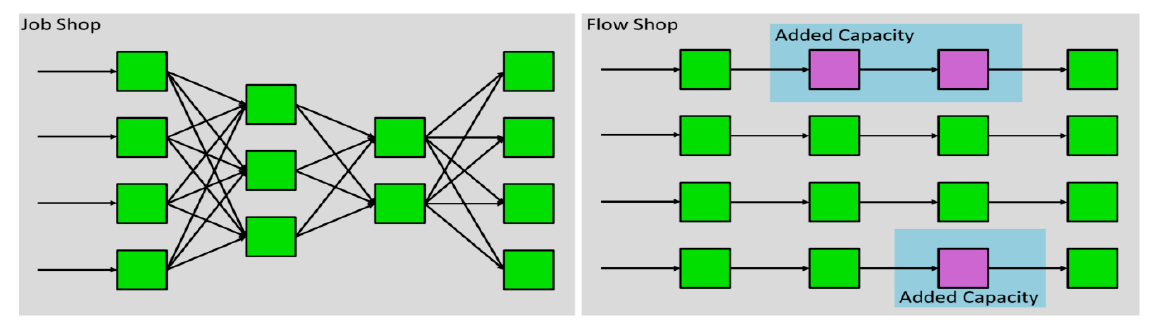
\includegraphics[width=0.9\linewidth]{flow_vs_job}
\end{center}
\begin{center}
\begin{tabularx}{\linewidth}{l X X}
\toprule
& \textbf{Flow shop} & \textbf{Job shop} \\
\midrule
Cheminement & \textbf{unique} : même séquence pour tous (M1 $\rightarrow$ M2 $\rightarrow$ M3) & \textbf{multiples} : séquence propre à chaque produit \\
Produits & standard, grande quantité & personnalisés, petites séries, forte variété \\
Flexibilité & faible & forte \\
Productivité & forte & faible \\
Implantation & \textbf{ligne de production} & sections homogènes \\
\bottomrule
\end{tabularx}
\end{center}
\par\begin{Arabic}
\textbf{بالدارجة:} \fr{flow shop} = كاع الدراجات كيدوزو من \textbf{نفس الطريق}. \fr{job shop} = كل دراجة عندها \textbf{الطريق ديالها}.
\end{Arabic}

\begin{exemple}
\begin{itemize}
\item Usine Lafarge-Holcim (ciment) $\rightarrow$ \textbf{flow shop}.
\item « Produit personnalisé à faible volume » $\rightarrow$ \textbf{job shop}.
\item « Les produits ont des cheminements différents » $\rightarrow$ \textbf{job shop}.
\item « Pour les petites séries : job shop ; pour les grandes séries : flow shop. » \vrai
\end{itemize}
\end{exemple}

\begin{note}
\textbf{Goulot d'étranglement} : la machine la plus \textbf{lente} de la ligne, qui ralentit tout.
\textbf{Flow shop with added capacity} : on ajoute des machines \textbf{en parallèle} au goulot pour augmenter la capacité.
\par\begin{Arabic}
بحال طريق فيها قنطرة ضيقة: كاع الطوموبيلات كيتسناو. الحل: نزيدو قنطرة أخرى بجانبها.
\end{Arabic}
\end{note}

\subsection*{3. Les implantations \quad (tombe à chaque test)}
\begin{center}
\begin{tabularx}{\linewidth}{>{\raggedright\arraybackslash}p{3.6cm} >{\raggedleft\arraybackslash}X >{\raggedright\arraybackslash}X}
\toprule
\textbf{Implantation} & \ar{\textbf{بالدارجة}} & \textbf{Quand ?} \\
\midrule
Position fixe & \ar{المنتوج \textbf{ما كيتحركش}، الماكينات والخدامة كيجيو عندو} & produit très \textbf{grand} : avion, navire, génie civil \\
Sections homogènes (fonctionnelle) & \ar{كنجمعو \textbf{الماكينات اللي كيديرو نفس الخدمة}: كاع الخراطات هنا، كاع الثقابات هنا} & \textbf{grande variété} (job shop) \\
Îlots / cellules & \ar{كنجمعو الماكينات \textbf{حسب عائلة المنتوج}، كل جزيرة مستقلة} & compromis flexibilité / productivité \\
En ligne (flow shop) & \ar{الماكينات فخط واحد بترتيب العمليات} & \textbf{un seul produit, grande quantité} \\
En U & \ar{الخط ملوي بحال حرف \fr{U} باش خدام واحد يخدم على بزاف ديال الماكينات} & réduire les déplacements \\
\bottomrule
\end{tabularx}
\end{center}

\begin{center}
\begin{tabular}{cc}
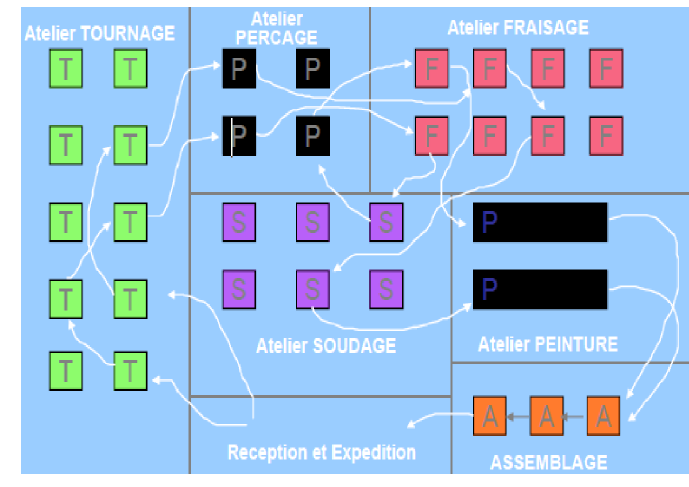
\includegraphics[width=0.46\linewidth]{sections_homogenes} &
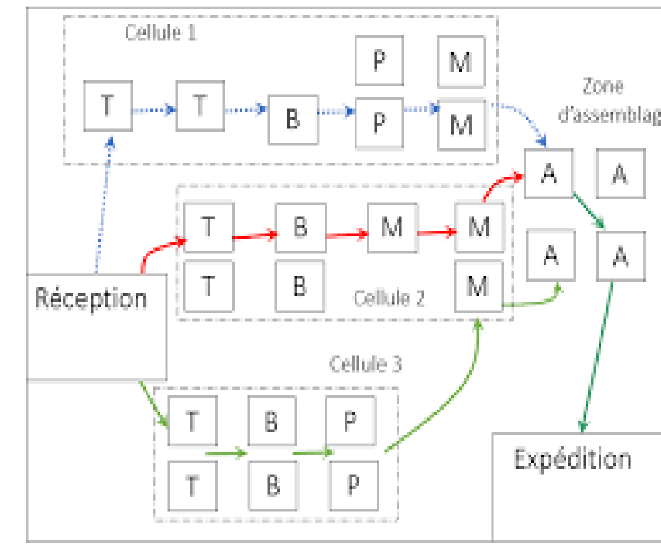
\includegraphics[width=0.46\linewidth]{ilots} \\
\small Sections homogènes : zones par \textbf{type de machine} &
\small Îlots : cellules par \textbf{famille de produits}
\end{tabular}

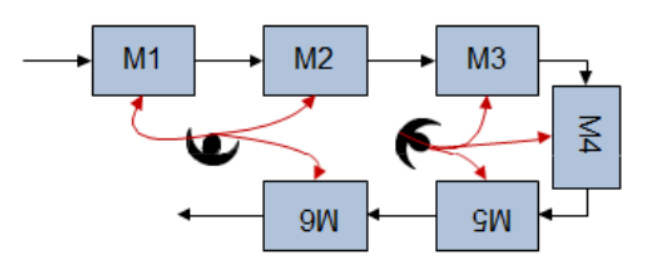
\includegraphics[width=0.45\linewidth]{implantation_U}\\
\small Implantation en U
\end{center}

\begin{note}
\par\begin{Arabic}
\textbf{ما تخلطش (غلطتي فيها فالـ QCM):}
\fr{Homogène} = «نفس النوع» ← كنجمعو حسب \textbf{الماكينة}.
\fr{Îlot} = جزيرة كتصنع \textbf{عائلة ديال المنتوجات} من البداية للنهاية.
\end{Arabic}
\end{note}

\textbf{Pourquoi l'îlot est meilleur que la section homogène ?} Moins de transports et de manutentions, moins d'en-cours et d'attentes, délais plus courts, équipes responsabilisées, automatisable.
\par\begin{Arabic}
فـ\fr{sections homogènes} المنتوج كيدور بزاف فالمعمل (شوف الفليشات فالتصويرة). فـ\fr{îlots} كلشي قريب.
\end{Arabic}

\begin{examen}
\begin{itemize}
\item Construction d'un avion $\rightarrow$ \textbf{implantation à produit fixe}.
\item Un seul produit en grandes quantités $\rightarrow$ \textbf{production en ligne}.
\item Acide phosphorique $\rightarrow$ \textbf{implantation en ligne} (flux continu).
\item Construction d'une nouvelle usine $\rightarrow$ \textbf{production par projet}.
\item Implantation physique d'un flow shop $\rightarrow$ \textbf{ligne de production}.
\item « On choisit une implantation fonctionnelle (sections homogènes) si le produit est diversifié. » \vrai
\item « Implantation en îlots pour un compromis entre flexibilité et productivité. » \vrai
\item Sections homogènes : « les machines sont regroupées en fonction de leurs fonctions similaires. » \vrai
\end{itemize}
\end{examen}
\begin{piege}
\begin{itemize}
\item « Implantation à produit fixe si les \textbf{machines} sont trop lourdes. » \faux \ \ar{(المنتوج هو اللي كبير، ماشي الماكينات)}
\item « Implantation en ligne si la diversité est élevée, en îlots si la qualité est requise. » \faux
\item « Flow shop : n'importe quelle implantation » ou « sections homogènes » \faux
\item « Le flow shop est plus flexible que le job shop. » \faux
\item « Le flow shop produit sur commande, le job shop en stock. » \faux
\end{itemize}
\end{piege}

\subsection*{4. Structure du produit : divergente ou convergente}
\begin{center}
\begin{tabularx}{\linewidth}{l >{\raggedleft\arraybackslash}X l}
\toprule
\textbf{Structure} & \ar{\textbf{بالدارجة}} & \textbf{Exemples} \\
\midrule
Divergente & \ar{مادة \textbf{وحدة} ← بزاف ديال المنتوجات (بحال شجرة كتتفرق)} & \textbf{lait}, \textbf{pétrole} \\
Convergente & \ar{بزاف ديال القطع ← منتوج \textbf{واحد} (كتتجمع)} & \textbf{voiture, avion, navire} \\
\bottomrule
\end{tabularx}
\end{center}
\begin{piege}
\begin{itemize}
\item « L'industrie pétrolière / laitière est à structure divergente. » \vrai
\item « La production d'un avion / d'un navire est à structure divergente. » \faux \ (convergente)
\end{itemize}
\end{piege}

\subsection*{5. Reconnaître les images (TD Q37)}
\par\begin{Arabic}
فالـ \fr{TD} كاين سؤال فيه تصاور خاصك تعرف شنو هي:
\end{Arabic}
\begin{itemize}
\item Machines reliées par des flèches \textbf{dans tous les sens} $\rightarrow$ \textbf{job shop}.
\item Zones « tournage / perçage / fraisage » avec des flèches longues $\rightarrow$ \textbf{sections homogènes}.
\item Cellules « Cellule 1, 2, 3 » avec T, B, M dedans $\rightarrow$ \textbf{îlots}.
\item Pièces rangées \textbf{par familles} dans des cases $\rightarrow$ \textbf{technologie de groupe}.
\item Tableau avec diagonale et zones grises « None / Dead zone » $\rightarrow$ \textbf{matrice produit / process} (partie 7).
\item Diagramme de Gantt (barres M1, M2, M3) $\rightarrow$ \textbf{rien de ces réponses}.
\end{itemize}

\begin{resume}
\begin{enumerate}
\item Flow shop = même chemin, grande quantité, ligne. Job shop = chemins différents, petite série.
\item Avion = position fixe ; un produit en masse = ligne ; diversité = sections homogènes ; compromis = îlots.
\item Pétrole et lait = divergente ; avion, navire, voiture = convergente.
\end{enumerate}
\end{resume}

\subsection*{Mini-QCM}
\begin{enumerate}
\item Lafarge-Holcim (ciment) : (a) job shop (b) flow shop (c) batch shop
\item Construction d'un avion : (a) en ligne (b) fonctionnelle (c) position fixe
\item Sections homogènes, machines regroupées : (a) par fonctions similaires (b) par famille de produits
\item Fabrication d'un navire : (a) divergente (b) convergente
\item Machine qui ralentit toute la ligne : (a) îlot (b) goulot d'étranglement
\end{enumerate}
{\small\textit{Réponses : 1-b, 2-c, 3-a, 4-b, 5-b.}}

%======================================================================
\partie{Partie 4c : Quand on produit ? (MTS / MTO / ATO / ETO)}

\begin{carte}
4a \checkmark\ $\rightarrow$ 4b \checkmark\ $\rightarrow$ \textbf{4c} $\rightarrow$ 5 $\rightarrow$ 6 $\rightarrow$ 7
\par\begin{Arabic}
\textbf{الدور ديال هاد الجزء:} بقا سؤال واحد: \textbf{واش كنصنعو قبل ما الزبون يطلب، ولا كنتسناو الطلبية ديالو؟}
\end{Arabic}
\end{carte}

\begin{center}
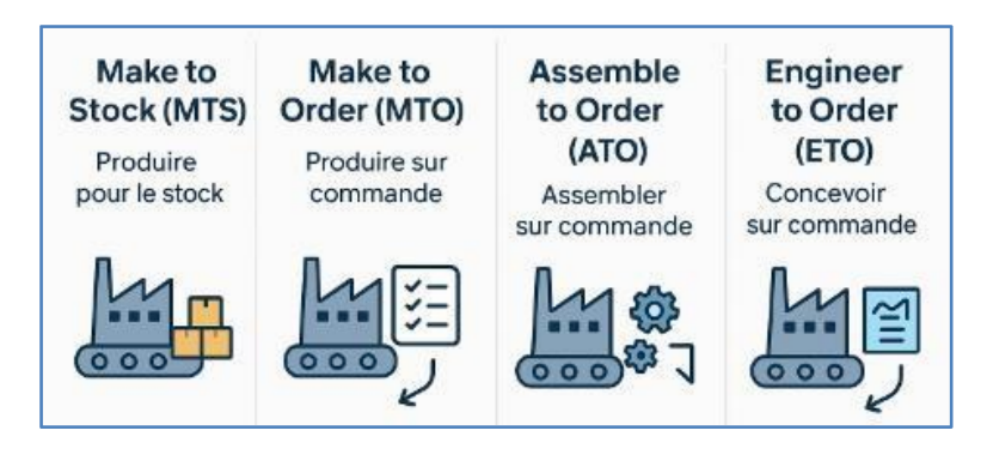
\includegraphics[width=0.75\linewidth]{mts_mto}
\end{center}

\begin{center}
\begin{tabularx}{\linewidth}{>{\raggedright\arraybackslash}p{3.6cm} >{\raggedleft\arraybackslash}X >{\raggedright\arraybackslash}X}
\toprule
\textbf{Mode} & \ar{\textbf{بالدارجة (مثال الساندويتش)}} & \textbf{Exemples d'examen} \\
\midrule
\textbf{MTS} Make to Stock & \ar{كنصنع \textbf{قبل} الطلبية وكنخزن: ساندويتش مغلف فالثلاجة} & vêtements prêt-à-porter, produit standard \\
\textbf{MTO} Make to Order & \ar{كنبدا نصنع \textbf{من بعد} الطلبية: كيوجدو ليك الساندويتش قدامك} & entreprise chimique (produits qui se conservent peu) \\
\textbf{ATO} Assemble to Order & \ar{القطع واجدين \textbf{من قبل}، كنركبهم \textbf{من بعد} الطلبية} & \\
\textbf{ETO} Engineer to Order & \ar{كنصمم \textbf{وكنصنع} من الصفر حسب الزبون: ساندويتش عملاق على المقاس} & machines industrielles sur mesure, produit spécifique \\
\bottomrule
\end{tabularx}
\end{center}

\begin{note}
\par\begin{Arabic}
\textbf{باش تتفكر:} \fr{\textbf{S}} = \fr{\textbf{S}tock} (كنخزن من قبل). \fr{\textbf{O}} = \fr{\textbf{O}rder} (كنتسنى الطلبية).
\textbf{التسليم من الأسرع للأبطأ:} \fr{MTS} ← \fr{ATO} ← \fr{MTO} ← \fr{ETO}.
\end{Arabic}
\end{note}

\begin{itemize}
\item \textbf{MTS = système push} (prévisions). On l'utilise quand le délai de fabrication \textbf{dépasse} le délai acceptable par le client ; la baisse des coûts exige une grande quantité.
\item \textbf{MTO = système pull} (commande). Approvisionnement + fabrication doivent tenir dans le délai du client ; avantage : \textbf{diminution des stocks}.
\end{itemize}

\begin{examen}
\begin{itemize}
\item « MTS produit des biens avant de recevoir une commande, tandis que MTO produit des biens en fonction des commandes reçues. » \vrai
\item « En MTO, le processus de fabrication ne commence que lorsque la commande client est reçue. » \vrai
\item « Une entreprise chimique attend que les clients passent commande (durée de conservation) : c'est MTO. » \vrai
\item « Produits spécifiques selon les exigences du client » $\rightarrow$ \textbf{ETO}.
\item « Un produit standard est en général fabriqué par le make to stock. » \vrai
\item « Les machines industrielles sur mesure sont souvent fabriquées en ETO. » \vrai
\item « Les vêtements prêt-à-porter sont produits en MTS. » \vrai
\end{itemize}
\end{examen}
\begin{piege}
\begin{itemize}
\item « En MTS, les commandes sont reçues avant que le produit ne soit fabriqué. » \faux
\item « En ETO, le délai de livraison est comparable à celui de l'ATO. » \faux \ \ar{(\fr{ETO} أطول بزاف)}
\item « MTO signifie Make to Stock et MTS Make to Order. » \faux
\item « MTO produit en grande quantité, MTS en petite quantité. » \faux
\end{itemize}
\end{piege}

\subsection*{Bonus : autonomie de l'entreprise (peu testé)}
\begin{itemize}
\item \textbf{Donneur d'ordres} (concepteur-fabricant) : conçoit et fabrique.
\item \textbf{Sous-traitant} : autonomie partielle, fabrique selon les plans du donneur d'ordres.
\item \textbf{Façonnier} : aucune autonomie, exécute seulement.
\end{itemize}

\begin{resume}
\begin{enumerate}
\item MTS = avant la commande (stock, push) ; MTO = après la commande (pull).
\item ATO = assemblage sur commande ; ETO = conception sur commande (le plus long).
\item Standard / prêt-à-porter = MTS ; sur mesure = ETO ; chimique périssable = MTO.
\end{enumerate}
\end{resume}

\subsection*{Mini-QCM}
\begin{enumerate}
\item Produits spécifiques selon le client : (a) MTS (b) MTO (c) ETO
\item Entreprise chimique qui attend les commandes : (a) MTS (b) MTO (c) ATO
\item Prêt-à-porter : (a) MTS (b) ETO (c) MTO
\item En ETO, le délai est comparable à l'ATO : (a) vrai (b) faux
\end{enumerate}
{\small\textit{Réponses : 1-c, 2-b, 3-a, 4-b.}}

%======================================================================
\partie{Partie 5 : Sélection du processus et calculs}

\begin{carte}
4 \checkmark\ $\rightarrow$ \textbf{Partie 5} $\rightarrow$ 6 $\rightarrow$ 7
\par\begin{Arabic}
\textbf{الدور ديال هاد الجزء:} فالجزء 4 شفنا \textbf{أنواع} المعامل. دابا خاصنا \textbf{نختارو} واحد منهم بـ\textbf{4 معايير}. وزيد عليهم \textbf{الحسابات} اللي كتطيح فكل امتحان.
\end{Arabic}
\end{carte}

\subsection*{1. Les 4 critères}
\begin{center}
\begin{tabularx}{\linewidth}{l X >{\raggedleft\arraybackslash}X}
\toprule
\textbf{Critère} & \textbf{Définition} & \ar{\textbf{بالدارجة}} \\
\midrule
Capacité de production & taux de production possible & \ar{شحال يقدر يصنع ماكسيمم} \\
Flexibilité & s'adapter à d'autres produits ou volumes & \ar{واش يقدر يتبدل بسهولة} \\
Tension du flux & temps à valeur ajoutée / temps total & \ar{شحال من الوقت خدام بصح} \\
Temps de cycle & durée totale, transport et manutention compris ; mesure la \textbf{réactivité} & \ar{الوقت كامل من البداية للنهاية} \\
\bottomrule
\end{tabularx}
\end{center}

\begin{examen}
\begin{itemize}
\item « La sélection du processus est effectuée lors de l'industrialisation d'un produit. » \vrai
\item « Elle doit tenir compte des données commerciales relatives au produit. » \vrai
\item « Elle doit tenir compte de la flexibilité et de la réactivité du système. » \vrai
\item « Elle est intimement liée à la conception du produit à réaliser. » \vrai
\item « La tension du flux mesure le pourcentage de la valeur ajoutée par rapport à tout le temps passé dans la production. » \vrai
\end{itemize}
\end{examen}
\begin{piege}
Toute phrase « ne doit \textbf{pas} tenir compte de\ldots{} » (données commerciales, quantité, variété, flexibilité) \faux
\end{piege}

\subsection*{2. Les calculs \quad (tombent à chaque test)}

\begin{tcolorbox}[colback=white,colframe=bleu,title=Formulaire,fonttitle=\bfseries]
\[
\text{Tension du flux} = \frac{\text{temps à valeur ajoutée}}{\text{temps total (VA + attentes + transport)}} \times 100
\]
\[
\text{Taux de charge} = \frac{\text{charge (ce qu'on doit / a produit)}}{\text{capacité disponible}} \times 100
\qquad
\text{Taux d'utilisation} = \frac{\text{temps de production}}{\text{temps disponible}} \times 100
\]
\end{tcolorbox}

\par\begin{Arabic}
\textbf{\fr{Tension du flux}:} المنتوج كيبقى فالمعمل وقت طويل، ولكن \textbf{ماشي كامل} كيتخدم عليه. بزاف ديال الوقت كيتسنى. التوتر كيقيس \textbf{شحال من الوقت مفيد}.

\textbf{\fr{Charge}} = الخدمة اللي \textbf{خاصك تدير} فعلا. \quad \textbf{\fr{Capacité}} = \textbf{الماكسيموم} اللي تقدر تدير.
\end{Arabic}

\begin{note}
\textbf{Méthode en 4 étapes :}
\begin{enumerate}
\item Repérer le \textbf{numérateur} (temps VA, ou production réelle) et le \textbf{dénominateur} (temps total, ou capacité).
\item Mettre tout dans la \textbf{même unité} (minutes !).
\item \textbf{Supprimer} les données inutiles (pièges : « 12 h par jour », « lead time 16 h »).
\item \textbf{Tronquer} : 33,33 $\rightarrow$ 33 ; 71,43 $\rightarrow$ 71 ; 66,9 $\rightarrow$ 66.
\end{enumerate}
\end{note}

\begin{exemple}
\textbf{Tension 1 (test 2023-24)} : séjour 8 h, dont 6 h de transformation. \quad $6/8 = \mathbf{75}$.

\textbf{Tension 2 (test 2024-25)} : VA = $45+30+50+35+20 = 180$ min ; attente 6 h = 360 min.\\
$180/(180+360) = 180/540 = 33{,}33 \rightarrow \mathbf{33}$.

\textbf{Tension 3} : VA = $20+40+30 = 90$ min ; attente 4 h 30 = 270 min. \quad $90/360 = \mathbf{25}$.

\textbf{Charge 1 (test 2023-24)} : capacité 500 pièces/jour, production 350 (la machine travaille 12 h : piège). \quad $350/500 = \mathbf{70}$.

\textbf{Charge 2 (TD Q2)} : 180 pièces $\times$ 2 min = 360 min ; machine 8 h = 480 min (lead time 16 h : piège). \quad $360/480 = \mathbf{75}$.

\textbf{Charge 3 (test 2024-25)} : 24 h à 100 pièces/h, arrêt 3 h, production 1\,500.\\
Capacité réelle = $(24-3)\times 100 = 2\,100$. \quad $1\,500/2\,100 = 71{,}43 \rightarrow \mathbf{71}$.

\textbf{Charge 4} : 20 h à 50 pièces/h, arrêt 4 h, production 600. \quad $600/((20-4)\times 50) = 600/800 = \mathbf{75}$.
\end{exemple}

\begin{piege}
\begin{itemize}
\item « La charge d'une ressource est la quantité \textbf{maximale} qu'elle peut traiter. » \faux
\item « La capacité est la quantité \textbf{réelle} à traiter. » \faux
\item « Lorsque la capacité dépasse la charge, la ressource est surchargée. » \faux \ \ar{(العكس: الحمل فايت القدرة)}
\item « Les opérateurs, les équipements et les outils sont tous appelés des ressources. » \vrai
\item « Taux d'utilisation = (temps de production / temps disponible) $\times$ 100. » \vrai
\end{itemize}
\end{piege}

\begin{alerte}
Test 2024-25 Q21 : la phrase « La charge d'une ressource est égale à la quantité réelle à traiter sur une période donnée » n'est \textbf{pas cochée} dans le corrigé, alors qu'elle est logique d'après le TD.
\par\begin{Arabic}
\textbf{النصيحة:} الجملة الوحيدة المضمونة هي « \fr{les ressources incluent les opérateurs, les équipements et les outils} ». إلا ما متأكدش من الباقي، ما تكوشيش (\fr{−0,5}).
\end{Arabic}
\end{alerte}

\begin{resume}
\begin{enumerate}
\item 4 critères : capacité, flexibilité, tension du flux, temps de cycle (réactivité).
\item Tension = VA / total ; taux de charge = charge / capacité disponible.
\item Même unité, enlever les données pièges, tronquer.
\end{enumerate}
\end{resume}

\subsection*{Mini-QCM}
\begin{enumerate}
\item Séjour 10 h dont 4 h de transformation : tension = ? \quad (a) 40 (b) 60 (c) 25
\item Capacité 400 pièces, production 300, machine 10 h/j : taux de charge = ? \quad (a) 30 (b) 75 (c) 133
\item 66,9 \% s'écrit : (a) 66 (b) 67
\item Le critère qui mesure la réactivité : (a) tension du flux (b) temps de cycle (c) capacité
\end{enumerate}
{\small\textit{Réponses : 1-a, 2-b, 3-a, 4-b.}}

%======================================================================
\partie{Partie 6 : Conception d'un système de production}

\begin{carte}
5 \checkmark\ $\rightarrow$ \textbf{Partie 6} $\rightarrow$ 7
\par\begin{Arabic}
\textbf{الدور ديال هاد الجزء:} اخترنا النوع ديال المعمل. دابا \textbf{كنبنيوه خطوة بخطوة}. وكنحددو \textbf{الوصفة} ديال تصنيع كل قطعة (\fr{gamme}).
\end{Arabic}
\end{carte}

\subsection*{1. Les 5 étapes pour construire l'usine}
\begin{center}
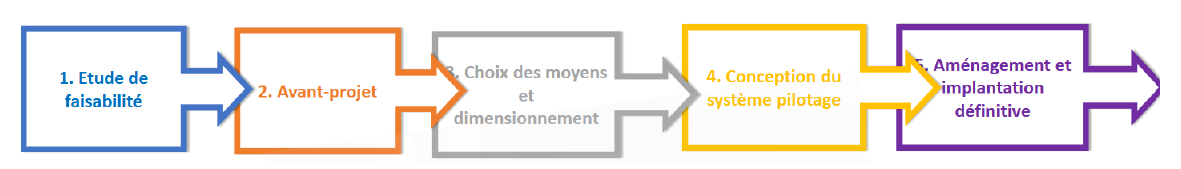
\includegraphics[width=0.85\linewidth]{etapes_systeme}
\end{center}
\begin{center}
\begin{tabularx}{\linewidth}{>{\raggedright\arraybackslash}p{3.6cm} >{\raggedleft\arraybackslash}X >{\raggedright\arraybackslash}X}
\toprule
\textbf{Étape} & \ar{\textbf{بالدارجة}} & \textbf{Mots-clés d'examen} \\
\midrule
1. Étude de faisabilité & \ar{واش ممكن؟ \textbf{نشريو ولا نصنعو؟}} & objectifs, contraintes, \textbf{alternatives (moulage / usinage)}, coût / planning \\
2. Avant-projet (APEF) & \ar{كنختارو الطريقة وكنحددو الماكينات \textbf{بشكل أولي}} & détails solution, \textbf{sélection des processus}, moyens achetés / conçus \\
3. Choix des moyens et dimensionnement & \ar{شحال من ماكينة؟ أشمن حجم؟ والأوراق الإدارية} & nombre et taille des stations, \textbf{équilibrage}, \textbf{dossier administratif (fournisseurs, appels d'offres, HSE)} \\
4. Conception du système de pilotage & \ar{البرنامج المعلوماتي اللي كيسير المعمل (\fr{MES})} & système informatique, \textbf{supervision, ordonnancement, gestion des capacités} \\
5. Aménagement et implantation définitive & \ar{كنركبو الماكينات فبلاصتهم النهائية} & \textbf{minimiser les manutentions}, suivi et contrôle de l'installation \\
\bottomrule
\end{tabularx}
\end{center}

\begin{note}
\par\begin{Arabic}
\textbf{باش تتفكر الترتيب:} واش ممكن؟ ← أشمن طريقة؟ ← شحال؟ ← البرنامج ← التركيب.
\end{Arabic}
\end{note}

\begin{exemple}
\textbf{Test 2022-23, Q16 à Q20} (association) : manutentions $\rightarrow$ \textbf{implantation} ; sélection des processus $\rightarrow$ \textbf{avant-projet} ; supervision / ordonnancement $\rightarrow$ \textbf{pilotage} ; alternatives moulage / usinage $\rightarrow$ \textbf{faisabilité} ; stations / équilibrage / HSE $\rightarrow$ \textbf{choix des moyens}.
\end{exemple}

\begin{piege}
\begin{itemize}
\item Le test 2022-23 écrit « étapes de la \textbf{conception de produits} » alors qu'il s'agit des étapes du \textbf{système de production}. \ar{ما تخلطش مع الجزء 3.}
\item « Avant-projet pour choisir de manière \textbf{définitive} les moyens. » \faux
\item « Avant-projet pour sélectionner le processus le plus adapté. » \vrai
\end{itemize}
\end{piege}

\subsection*{2. La gamme de fabrication}
\par\begin{Arabic}
\fr{\textbf{Gamme}} = \textbf{الترتيب ديال العمليات} باش تصنع قطعة. بحال وصفة الطبخ: أولا خرط، من بعد ثقب، من بعد صقل… كاينين \textbf{جوج طرق}:
\end{Arabic}
\begin{center}
\begin{tabularx}{\linewidth}{l X X}
\toprule
& \textbf{Générative} & \textbf{Déductive} \\
\midrule
Principe & nouvelle gamme \textbf{à partir de zéro}, depuis le dessin de la pièce & on part de l'\textbf{existant} : une \textbf{gamme type} de la même famille qu'on personnalise \\
Outil & règles, systèmes experts, \textbf{expertise poussée} & \textbf{technologie de groupe (TG)}, codification (code CETIM / PMG) \\
Quand ? & \textbf{diversité importante} & \textbf{grande quantité, petite variété} \\
Étapes & surfaces $\rightarrow$ formes $\rightarrow$ entités d'usinage $\rightarrow$ phases $\rightarrow$ ordonnancement & codification $\rightarrow$ mémoire de l'entreprise $\rightarrow$ gamme type $\rightarrow$ opérations complémentaires \\
\bottomrule
\end{tabularx}
\end{center}

\begin{note}
\par\begin{Arabic}
\textbf{القاعدة الوحيدة (غلطتي فيها فالـ QCM):}
\end{Arabic}
\centering
\textbf{\textcolor{bleu}{D}éductive = \textcolor{bleu}{D}éjà existant = TG = gamme type = peu de variété}\\
\textbf{Générative = générer du neuf = beaucoup de variété}
\end{note}

\subsection*{3. Technologie de groupe (TG)}
\par\begin{Arabic}
\textbf{الفكرة:} كنجمعو القطع \textbf{الشبيهة} فـ\textbf{عائلات}، وكنعطيو لكل قطعة \textbf{كود} حسب الشكل والقياسات. والعائلات كتتصنع فنفس الجزيرة (\fr{îlot}) ديال الجزء \fr{4b}.
\end{Arabic}
\begin{examen}
\begin{itemize}
\item « Se base sur la codification morpho-dimensionnelle des produits. » \vrai
\item « Permet d'associer à un produit une gamme type et des outillages de fabrication. » \vrai
\item « Permet de regrouper des produits similaires en familles pour simplifier la production. » \vrai
\item « Favorise l'organisation des machines par familles de produits similaires. » \vrai
\item « Réduit les coûts en standardisant les processus pour des produits similaires. » \vrai
\item « Optimise le temps de changement d'outillage. » \vrai
\item « L'approche déductive utilise une base de données d'anciennes gammes. » \vrai
\item « Une cellule flexible d'usinage utilise la technologie de groupe. » \vrai
\item Démarche générative : « lors de l'élaboration de l'APEF d'une pièce » et « pour concevoir une gamme d'usinage d'une pièce mécanique ». \vrai
\end{itemize}
\end{examen}
\begin{piege}
\begin{itemize}
\item « La TG n'est pas compatible avec les approches productiques modernes. » \faux
\item « La TG n'a aucun rapport avec l'implantation des machines. » \faux
\item « L'approche \textbf{générative} fait appel à la TG / repose sur la TG. » \faux
\item « La générative consiste à élaborer une \textbf{gamme type}. » \faux
\item « La \textbf{déductive} peut être utilisée lorsque la diversité est très importante. » \faux
\item « On peut adopter une démarche générative pour mettre en œuvre la TG. » \faux
\item « La déductive / générative sert à concevoir un système informatique de pilotage. » \faux
\item « Il existe deux approches : la TG et la TGAO. » \faux
\item « La déductive est basée sur la conception automatisée, sans intervention humaine. » \faux
\item « La TG réduit la variété des produits » / « utilise des robots ». \faux
\end{itemize}
\end{piege}

\begin{resume}
\begin{enumerate}
\item Faisabilité $\rightarrow$ avant-projet (préliminaire) $\rightarrow$ moyens $\rightarrow$ pilotage (MES) $\rightarrow$ implantation.
\item Générative = de zéro, grande diversité. Déductive = existant, TG, gamme type.
\item TG = familles, codification morpho-dimensionnelle, gamme type, outillages.
\end{enumerate}
\end{resume}

\subsection*{Mini-QCM}
\begin{enumerate}
\item « Minimiser les manutentions » : (a) faisabilité (b) avant-projet (c) implantation
\item « Supervision, ordonnancement, gestion des capacités » : (a) choix des moyens (b) pilotage (c) avant-projet
\item La générative : (a) fait appel à la TG (b) diversité importante (c) gamme type
\item La déductive : (a) diversité très importante (b) fait appel à la TG (c) système de pilotage
\item « Stations, équilibrage, appels d'offres, HSE » : (a) faisabilité (b) choix des moyens (c) implantation
\end{enumerate}
{\small\textit{Réponses : 1-c, 2-b, 3-b, 4-b, 5-b.}}

%======================================================================
\partie{Partie 7 : Industrialisation et cycle de vie}

\begin{carte}
6 \checkmark\ $\rightarrow$ \textbf{Partie 7} $\rightarrow$ fin du chapitre 1
\par\begin{Arabic}
\textbf{الدور ديال هاد الجزء:} عندنا دراجة تجريبية وعندنا المعمل. دابا كنحولو الدراجة التجريبية لـ\textbf{آلاف الدراجات} مصنوعين مزيان وبثمن معقول.
\end{Arabic}
\end{carte}

\subsection*{1. Définition}
\par\begin{Arabic}
\textbf{بالدارجة:} نحولو فكرة ولا نموذج تجريبي لمنتوج \textbf{كيتصنع بسهولة، صالح، ورخيص} (\fr{fabriquable, fiable, compétitif}).
\end{Arabic}
\begin{examen}
\begin{itemize}
\item « L'industrialisation est le processus de choix et mise en place d'un système de production adéquat pour un produit donné. » \vrai
\item « L'industrialisation d'un produit est le fait de concevoir et mettre en place un système de production adéquat. » \vrai
\item « Le développement de produit est le processus de conception d'un nouveau produit, de l'idée jusqu'au lancement. » \vrai
\item « Un avant-projet est élaboré pour sélectionner le processus le plus adapté au produit. » \vrai
\end{itemize}
\end{examen}

\subsection*{2. Le grand piège « Lors de l'industrialisation\ldots{} » \quad (dans les 3 tests)}
\begin{center}
\begin{tabularx}{\linewidth}{X c}
\toprule
\textbf{Phrase} & \textbf{Réponse} \\
\midrule
« Il faut concevoir et mettre en place un système de production adéquat » & \vrai \\
« Job shop si les produits ont des cheminements différents » / « pour les petites séries » & \vrai \\
« Un avant-projet pour sélectionner le processus » & \vrai \\
« On peut \textbf{acheter} les moyens si on doit produire de \textbf{grandes quantités} » & \faux \\
« Les moyens sont achetés si le produit est destiné à une production \textbf{en masse} » & \faux \\
« Il faut \textbf{concevoir} les moyens si la \textbf{diversité} est élevée » & \faux \\
« Les moyens doivent \textbf{toujours} être développés en interne » & \faux \\
\bottomrule
\end{tabularx}
\end{center}

\begin{alerte}
Le TD coche : « système \textbf{flexible} $\rightarrow$ moyens généralement \textbf{conçus} » et « système \textbf{dédié} $\rightarrow$ moyens généralement \textbf{achetés} ».
\par\begin{Arabic}
\textbf{الفرق فالكلمات:} الـ \fr{TD} كيهضر على نوع النظام (\fr{flexible / dédié}) ← صحيح. الامتحانات كتهضر على \fr{quantité / diversité} ← ديما غالط. \textbf{ركز على الكلمة.}
\end{Arabic}
\end{alerte}

\subsection*{3. Les 3 sections de l'industrialisation}
\begin{enumerate}
\item \textbf{Soutien à la conception} : intégrer la fabrication dès la conception $\rightarrow$ \textbf{DFMA} (Design For Manufacturing and Assembly).
\item \textbf{Méthodes et préparation} : gammes, outillages, machines, séquences pour passer du prototype à la série.
\item \textbf{Amélioration continue} : réduire les gaspillages $\rightarrow$ \textbf{Lean, Kaizen, 5S}.
\end{enumerate}

\subsection*{4. Ingénierie simultanée (intégrée / concourante)}
\par\begin{Arabic}
بدل ما كل قسم يخدم \textbf{وحدو ومن بعد} يعطي الخدمة للآخر، \textbf{كاع الأقسام كيخدمو مع بعض فنفس الوقت} من البداية (التصميم، الإنتاج، الجودة، المشتريات، اللوجستيك).
\end{Arabic}
\begin{note}
Ce n'est \textbf{pas une section} : c'est une \textbf{approche organisationnelle transversale}.\\
\textbf{Vision métier} : chaque service voit sa fonction. \textbf{Vision projet} : tout le cycle de vie, du besoin client au marché.
\end{note}

\subsection*{5. Matrice produit-processus (Hayes \& Wheelwright)}
\begin{center}
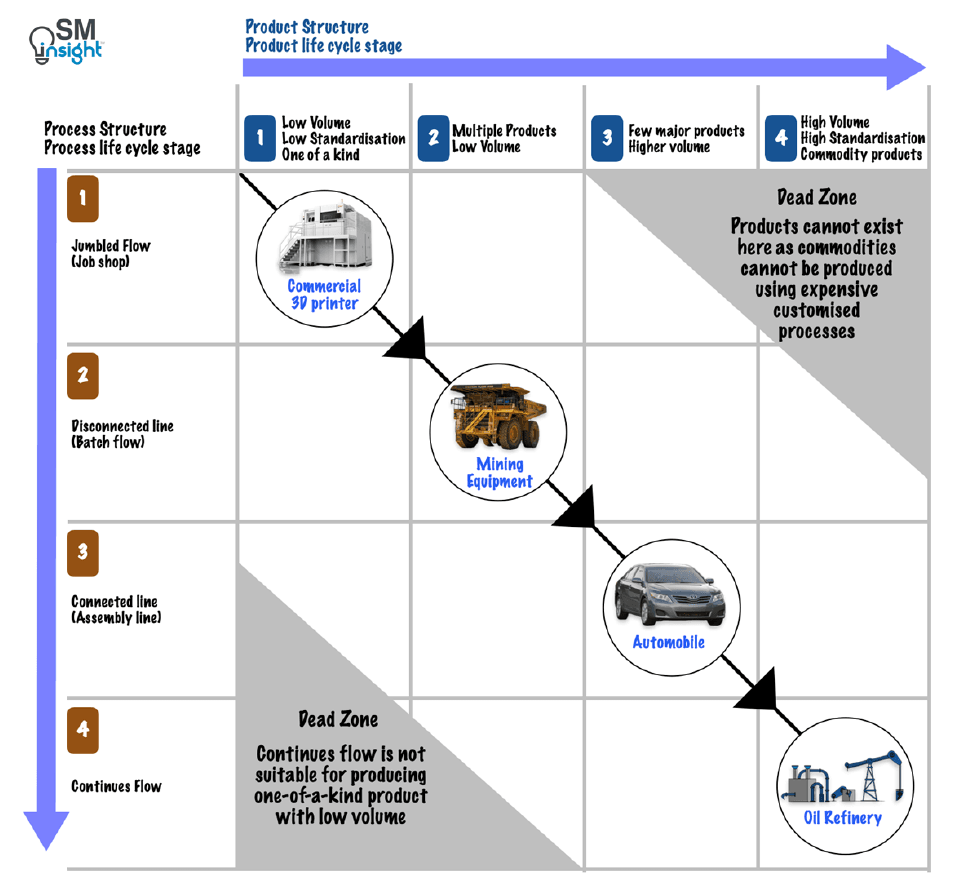
\includegraphics[width=0.7\linewidth]{matrice_hw}
\end{center}
\par\begin{Arabic}
\textbf{الفكرة:} المعمل خاصو \textbf{يتبدل مع حياة المنتوج}. كلما المنتوج كيكبر ويستقر، كلما المعمل كيولي أوتوماتيكي ومنتج.
\end{Arabic}
\begin{center}
\begin{tabular}{llll}
\toprule
\textbf{Phase du produit} & \textbf{Processus} & \textbf{Volume} & \textbf{Exemple} \\
\midrule
Introduction & projet / job shop & prototype, unitaire & imprimante 3D \\
Croissance & par lots (batch) & petite série & engins miniers \\
Maturité & en ligne & grande série & automobile \\
Déclin & continu & masse & raffinerie \\
\bottomrule
\end{tabular}
\end{center}
\par\begin{Arabic}
\textbf{الخط المائل} = الاختيار الصحيح. \textbf{المثلثات الرمادية} (\fr{dead zones}) = اختيارات غالطة:
فوق ليمن: ما تقدرش تصنع منتوج بالكمية الضخمة بطريقة يدوية غالية. لتحت ليسر: ما تقدرش تدير خط مستمر لقطعة وحدة.
\end{Arabic}

\subsection*{6. Questions de raisonnement sur les coûts (test 2024-25)}
\begin{examen}
\begin{itemize}
\item Économies d'échelle $\rightarrow$ \textbf{production en masse} (pas par lot).
\item « Un système flexible augmente les coûts d'investissement initial, mais permet de mieux contrôler les coûts de production en cas de baisse de la demande. » \vrai
\item « Une ligne dédiée est moins coûteuse en phase de maturité mais devient plus coûteuse en phase de déclin en raison de son manque de flexibilité. » \vrai
\item « En lancement, les coûts d'investissement sont élevés ; en maturité, les économies d'échelle réduisent ces coûts. » \vrai
\item « Les coûts restent identiques quelle que soit la phase. » \faux
\end{itemize}
\end{examen}

\begin{resume}
\begin{enumerate}
\item Industrialisation = choix et mise en place d'un système de production adéquat.
\item « Acheter si grandes quantités » et « concevoir si diversité » = toujours FAUX aux tests.
\item L'usine évolue avec le produit : job shop $\rightarrow$ lots $\rightarrow$ ligne $\rightarrow$ continu.
\end{enumerate}
\end{resume}

\subsection*{Mini-QCM}
\begin{enumerate}
\item Lors de l'industrialisation : (a) acheter si grandes quantités (b) job shop si cheminements différents (c) concevoir si diversité élevée
\item Économies d'échelle : (a) production en masse (b) production par lot
\item Automobile (maturité) : (a) job shop (b) en ligne (c) continu
\item Intégrer la fabrication dès la conception : (a) DFMA (b) Kaizen (c) 5S
\end{enumerate}
{\small\textit{Réponses : 1-b, 2-a, 3-b, 4-a.}}

%======================================================================
\partie{Bilan : à relire la veille de l'examen}

\subsection*{Top 15 des pièges du chapitre 1}
\begin{enumerate}
\item « uniquement » dans une définition $\rightarrow$ FAUX.
\item Tiré / poussé / tendu ne sont \textbf{pas} des flux de l'entreprise (ce sont MTO / MTS / JIT).
\item Time to market : il faut le \textbf{réduire}.
\item Cycle de vie : \textbf{développement}, lancement, croissance, maturité, déclin.
\item Préliminaire = architecture, \textbf{après} le concept.
\item Alpha = autre procédé ; présérie = procédé final.
\item Innovation = invention adoptée par le marché (pas l'inverse).
\item Variété $\rightarrow$ flexibilité ; quantité $\rightarrow$ productivité.
\item Sections homogènes = même type de machine ; îlots = famille de produits.
\item Position fixe = le \textbf{produit} est grand (pas les machines lourdes).
\item Avion, navire = convergente ; pétrole, lait = divergente.
\item MTS = avant commande ; ETO = le plus long.
\item Déductive = TG = gamme type ; générative = diversité.
\item Avant-projet = choix \textbf{préliminaire}, jamais définitif.
\item « Acheter si grandes quantités », « concevoir si diversité » $\rightarrow$ FAUX.
\end{enumerate}

\subsection*{Mes points faibles (d'après mes QCM)}
\par\begin{Arabic}
\begin{itemize}
\item \fr{ISO 45001} = \fr{santé et sécurité} (ماشي \fr{9001}).
\item الفلوكس ديال المعلومات كيبدا من \textbf{الزبون}.
\item \fr{Générative} vs \fr{déductive}: \fr{D = Déjà existant}.
\item \fr{Sections homogènes} vs \fr{îlots}.
\end{itemize}
\end{Arabic}

\subsection*{Checklist}
\begin{itemize}[label=$\square$]
\item Je sais définir produit, processus, système de production, et repérer « uniquement ».
\item Je connais les 6 étapes du NPD et la différence concept / préliminaire / détaillée.
\item Je distingue maquette, alpha, présérie.
\item Je sais choisir l'implantation pour : avion, ciment, acide phosphorique, produit varié, compromis.
\item Je distingue flow shop / job shop, divergente / convergente.
\item Je sais classer un exemple en MTS, MTO, ATO, ETO.
\item Je sais calculer tension du flux et taux de charge, avec troncature.
\item Je connais les 5 étapes de conception du système et leurs mots-clés.
\item Je distingue générative / déductive et je connais les phrases vraies sur la TG.
\item Je connais le piège « lors de l'industrialisation » et la matrice de Hayes \& Wheelwright.
\end{itemize}

\end{document}
